\chapter{Das expandierende Newtonsche Universum}

\lectureoverview{Die moderne Kosmologie beginnt damit, das Universum selbst als physikalisches System zu behandeln. Ausgehend von großräumiger Isotropie und Homogenität führen wir ein mitbewegtes Koordinatengitter ein und beschreiben seine Bewegung durch einen einzigen Skalenfaktor \(a(t)\). Der Schalentheorem von Newton reduziert das gravitative Vielteilchenproblem dann auf eine Gleichung für \(a(t)\). Die Energieerhaltung unterscheidet zwischen Universen, die wieder kollabieren, einem kritischen Universum und ewig expandierenden Universen. Im kritischen, materiedominierten Fall erhält man die erste Friedmann-Gleichung und das Gesetz \(a(t)\propto t^{2/3}\).}

\section{Als die Kosmologie zur Physik wurde}

Die Kosmologie ist ein altes Fach, doch die quantitative Kosmologie ist jung. Für unsere Zwecke müssen wir nicht bei den Griechen beginnen. Sinnvolle historische Ausgangspunkte sind Hubbles Entdeckung der kosmischen Expansion im zweiten Viertel des zwanzigsten Jahrhunderts und, später, die Erkenntnis, dass der Mikrowellenhintergrund mit einer Temperatur von ungefähr drei Kelvin ein Überbleibsel eines heißen frühen Universums ist.

Bevor Messungen präzise wurden, glich ein großer Teil der Astronomie zwangsläufig der Naturgeschichte. Man entdeckte einen ungewöhnlichen Stern, klassifizierte eine eigenartige Galaxie, maß, was sich messen ließ, und stellte einen Katalog von Objekten zusammen. Diese Objekte waren selbstverständlich physikalische Systeme: Sie besaßen Drehimpuls, enthielten chemische Elemente und gehorchten den Gesetzen der Mechanik. Die entscheidende Veränderung bestand darin, das \emph{gesamte Universum} als ein einziges physikalisches System zu behandeln, das durch Gleichungen beschrieben wird, die genau genug sind, um sich an Beobachtungen messen zu lassen.

Darum geht es hier. Wir werden nicht bloß die Inhalte des Universums aufzählen, sondern nach seinen Variablen, seiner Bewegung und seinem dynamischen Gesetz fragen. Gleichungen sind kein nachträglicher Schmuck der Kosmologie. Sie sind das Mittel, mit dem das Universum zu einem physikalischen Problem wird.

Historisch wurde das expandierende Universum im Rahmen der allgemeinen Relativitätstheorie verstanden. Logisch gesehen ist jedoch ein großer Teil der ersten Argumentation Newtonsch. Ein Physiker des siebzehnten Jahrhunderts hätte ein bemerkenswert gutes Modell herleiten können, wenn er die richtige großräumige Bewegung vorausgeahnt hätte. Der Ausgangspunkt bei Newton soll die Relativitätstheorie nicht ersetzen, sondern die Mechanik herausarbeiten, die diese später geometrisch neu ordnet.

\section{Isotropie, Homogenität und das kosmologische Prinzip}

Der erste Schritt ist die Beobachtung. Auf ausreichend großen Skalen ist das Universum näherungsweise \emph{isotrop}: Wenn man Himmelsbereiche mittelt und den Vordergrund der Milchstraße hinter sich lässt, sieht es in jeder Richtung weitgehend gleich aus. Damit ist keine exakte Gleichförmigkeit gemeint. Ein direkter Blick auf einen nahen Stern unterscheidet sich von einem Blick in einen leeren Himmelsbereich, und die Materieverteilung weist tatsächlich Strukturen auf. Isotropie ist eine gemittelte Aussage über große Skalen.

Homogenität ist eine andere Aussage. Sie besagt, dass das gemittelte Universum von Ort zu Ort gleich ist. Ein Beobachter in vielen Galaxien Entfernung sollte nach derselben großräumigen Mittelung näherungsweise dieselbe Art von Universum sehen wie wir.

In erster Näherung kann eine Galaxie schlicht als Massepunkt behandelt werden. Das sichtbare Universum enthält ungefähr
\begin{equation}
N_{\rm gal}\sim 10^{11}
\end{equation}
Galaxien, jede mit etwa \(10^{11}\) Sternen. Das ergibt ungefähr \(10^{22}\) Sterne. Nimmt man als bewusst grobe Größenordnungsschätzung zehn Planeten pro Stern an, erhält man \(10^{23}\) Planeten – bemerkenswerterweise nahe an einem Mol Planeten. Diese Zahlenschätzung gehört nicht zur Dynamik, gibt aber eine Vorstellung von der Größe des idealisierten Systems.

\begin{classroomqa}
\classquestion{Wie viele Galaxien gibt es größenordnungsmäßig im beobachtbaren Universum?}
\lecturerresponse{Etwa hundert Milliarden, also \(10^{11}\). Bei ungefähr \(10^{11}\) Sternen pro Galaxie entspricht das etwa \(10^{22}\) Sternen im sichtbaren Universum. Diese Größenordnungsschätzungen sollte man im Hinterkopf behalten, auch wenn in der folgenden Rechnung jede Galaxie durch einen einzigen Massepunkt ersetzt wird. \lecturetimestamp{00:06:08--00:07:05}}
\end{classroomqa}

Warum legt Isotropie um uns herum Homogenität nahe? Stellen wir uns eine isotrope Verteilung vor, die \emph{nicht} homogen ist. Ihre Dichte müsste sich mit der Entfernung von uns ändern, dabei aber unabhängig von der Richtung bleiben: Sie würde also konzentrische Schalen um unseren Standort bilden. Ein Beobachter, der vom gemeinsamen Zentrum versetzt wäre, würde keine Isotropie mehr sehen. Es gibt daher zwei Möglichkeiten:
\begin{enumerate}
\item Wir befinden uns in einem ausgezeichneten Zentrum, um das herum das Universum angeordnet ist; oder
\item die großräumige Verteilung ist näherungsweise homogen, sodass kein Ort ausgezeichnet ist.
\end{enumerate}
Die zweite Möglichkeit ist die sparsamere Annahme. Isotropie führt zusammen mit der Weigerung, uns selbst eine privilegierte kosmische Position zuzuschreiben, zur Homogenität.

\begin{classroomqa}
\classquestion{Welche Form könnte eine isotrope, aber inhomogene Verteilung haben?}
\lecturerresponse{Ihre Variation könnte nur von unserer Entfernung abhängen und so ein schalenförmiges Muster mit unserem Standort als Zentrum bilden. Bewegt sich der Beobachter von diesem Zentrum weg, ist das Muster nicht mehr isotrop. Solange unser Standort nicht besonders ist, spricht Isotropie daher für Homogenität. \lecturetimestamp{00:07:06--00:08:54}}
\end{classroomqa}

Die gemeinsame Annahme heißt \emph{kosmologisches Prinzip}: Auf ausreichend großen Skalen ist das Universum räumlich homogen und isotrop. Die Bezeichnung als Prinzip beweist nichts. Historisch übernahmen Kosmologen diese Annahme, bevor Beobachtungen sie überzeugend stützten. Ihr Ansehen verdankt sie ihrem empirischen Erfolg.

Auch ist Homogenität nicht exakt. Galaxien bilden Haufen und Superhaufen, und seit Langem wird über Strukturen diskutiert, die sich über sehr große Teile des sichtbaren Himmels erstrecken. Die angemessene Aussage lautet, dass sich Fluktuationen herausmitteln, wenn das Mittelungsgebiet hinreichend groß ist---in dieser Einführung in der Größenordnung von einigen hundert Millionen bis ungefähr einer Milliarde Lichtjahren. Die Skala lässt sich anhand von Beobachtungen präzisieren; die Methode besteht darin, so lange gröber zu mitteln, bis lokale Strukturen die Beschreibung nicht mehr dominieren.

\begin{classroomqa}
\audiencequestion{Liefert die Gleichförmigkeit der kosmischen Mikrowellenhintergrundstrahlung einen Beleg für das kosmologische Prinzip?}
\lecturerresponse{Ja. Das kosmologische Prinzip wurde vorgeschlagen, bevor es starke Beobachtungsgründe dafür gab. Später zeigte die Mikrowellenhintergrundstrahlung jedoch, dass das ursprüngliche Universum außerordentlich glatt war. Galaxien und Haufen entstanden aus kleinen Abweichungen von diesem glatten Zustand; sie beseitigen nicht die großräumigen Belege dafür. \lecturetimestamp{00:10:53--00:11:43}}
\end{classroomqa}

\section{Ein mit den Galaxien mitbewegtes Gitter}

Sobald die beobachtungsbasierte Näherung gewählt ist, müssen wir Variablen festlegen. Auf die Frage „Was ist der erste Schritt bei der Formulierung eines physikalischen Problems?“ lautet eine Antwort aus dem Hörsaal: die Variablen kennen; die traditionelle Antwort lautet: den Bleistift spitzen. Hier findet man die entscheidende Variable, indem man die Koordinaten geschickt wählt.

Stellen wir uns ein dreidimensionales Gitter mit den Bezeichnungen \(x,y,z\) vor. Diese Bezeichnungen müssen keine in Metern gemessenen Abstände sein. Es sind Koordinatenwerte. Wir wählen das Gitter so, dass jede Galaxie nach dem Herausmitteln kleiner Pekuliarbewegungen an einem festen Gitterpunkt bleibt. Die Galaxien sind dann \emph{mitbewegend}.

Eine solche Wahl wäre nutzlos, wenn sich die Galaxien zufällig bewegten. Die Beobachtungen zeigen stattdessen eine kohärente großräumige Bewegung. Benachbarte Gitterzellen können expandieren oder sich zusammenziehen, aber dieselbe Expansion oder Kontraktion findet überall statt. Daher lassen sich alle physikalischen Abstände als ein gemeinsamer, zeitabhängiger Skalenfaktor mal einem festen Koordinatenabstand schreiben.

Für zwei Galaxien \(A\) und \(B\) gilt:
\begin{equation}
\begin{aligned}
d_{AB}(t)&=a(t)\,\Delta\chi_{AB},\\
\Delta\chi_{AB}
&=\sqrt{(x_A-x_B)^2+(y_A-y_B)^2+(z_A-z_B)^2}.
\end{aligned}
\label{eq:c01-physical-distance}
\end{equation}
Unterscheiden sie sich nur in der \(x\)-Koordinate, vereinfacht sich dies zu
\begin{equation}
d_{AB}(t)=a(t)\,\Delta x_{AB}.
\end{equation}
Die Funktion \(a(t)\) ist der \emph{Skalenfaktor}. Seine absolute Normierung ist konventionell: Multipliziert man alle mitbewegten Koordinaten mit einer Konstanten und dividiert \(a\) durch dieselbe Konstante, ändert sich kein physikalischer Abstand. Verhältnisse wie \(a(t_2)/a(t_1)\) und Ableitungen dividiert durch \(a\) enthalten die physikalische Information.

Leiten wir Gleichung~\eqref{eq:c01-physical-distance} ab. Der mitbewegte Abstand ist fest, also gilt
\begin{equation}
v_{AB}=\dot a\sqrt{(\Delta x)^2+(\Delta y)^2+(\Delta z)^2}.
\end{equation}
Dividieren wir durch den physikalischen Abstand, erhalten wir
\begin{equation}
\frac{v_{AB}}{d_{AB}}=\frac{\dot a}{a}\equiv H(t),
\label{eq:c01-hubble-parameter}
\end{equation}
oder
\begin{equation}
\boxed{v_{AB}=H(t)d_{AB}.}
\label{eq:c01-hubble-law}
\end{equation}
Dies ist das Hubble-Gesetz für die idealisierte homogene Strömung.

Die Bezeichnung „Hubble-Konstante“ kann irreführend sein. Zu einem gegebenen kosmischen Zeitpunkt gilt derselbe Wert von \(H\) an jedem Ort des homogenen Modells, aber \(H(t)\) ändert sich im Allgemeinen mit der Zeit. Räumliche Universalität bedeutet keine zeitliche Konstanz.

\begin{classroomqa}
\audiencequestion{Haben wir mit der Darstellung jedes Abstands als gemeinsamer Faktor \(a(t)\) mal einem festen Koordinatenabstand das Hubble-Gesetz bereits vorausgesetzt?}
\lecturerresponse{Der Ansatz ist gewiss durch Hubbles Beobachtung motiviert; ohne Belege für eine kohärente Rezession wäre er kaum naheliegend. Sein Nutzen besteht darin, diese Beobachtungen zu ordnen. Statt jeder Galaxie eine unabhängige Geschwindigkeit zuzuweisen, beschreibt man ein einziges expandierendes Gitter. Ist diese Beschreibung einmal gewählt, folgt die Proportionalität \(v=Hd\) durch Differentiation. \lecturetimestamp{00:24:20--00:25:33}}
\end{classroomqa}

Dieselbe Bewegung lässt sich auf zwei Arten beschreiben. Man kann sagen, dass sich die Galaxien im Raum voneinander entfernen, oder dass die Galaxien an festen mitbewegten Positionen bleiben, während sich das Gitter---und damit der physikalische Raum zwischen ihnen---ausdehnt. Auf dieser Stufe sind dies zwei Koordinatenbeschreibungen derselben Mathematik. Die Sprache vom expandierenden Raum wird in der allgemeinen Relativitätstheorie besonders natürlich sein. Beobachtungen können jedoch zwei Beschreibungen nicht unterscheiden, wenn beide zu jeder Zeit dieselben physikalischen Abstände angeben.

\section{Massenbilanz in einer mitbewegten Zelle}

Bevor wir die Gravitation einführen, verfolgen wir die Masse. Betrachten wir eine kleine Koordinatenzelle mit dem Koordinatenvolumen
\begin{equation}
\Delta V_{\rm com}=\Delta x\,\Delta y\,\Delta z.
\end{equation}
Sie muss dennoch groß genug sein, um viele Galaxien zu enthalten, sodass sich lokale Fluktuationen herausmitteln lassen. Sei \(\nu\) die Masse pro Einheit des mitbewegten Koordinatenvolumens. Die Masse in der Zelle ist
\begin{equation}
\Delta M=\nu\,\Delta x\,\Delta y\,\Delta z.
\label{eq:c01-comoving-mass}
\end{equation}
Da sich die Zelle mit der Materie bewegt, durchquert im idealen Strömungsbild keine Galaxie ihren Rand, und \(\Delta M\) bleibt konstant.

Jede physikalische Kante ist um den Faktor \(a(t)\) länger als die entsprechende Koordinatenkante. Das physikalische Volumen ist daher
\begin{equation}
\Delta V_{\rm phys}=a^3(t)\,\Delta x\,\Delta y\,\Delta z.
\end{equation}
Die physikalische Massendichte ist
\begin{equation}
\boxed{\rho(t)=\frac{\Delta M}{\Delta V_{\rm phys}}=\frac{\nu}{a^3(t)}.}
\label{eq:c01-density-dilution}
\end{equation}
Drucklose Materie wird durch die Expansion gemäß \(a^{-3}\) verdünnt; bei der Kontraktion wird sie nach demselben Gesetz konzentriert.

Bis hierher haben wir keine dynamischen Annahmen gemacht. Wir haben euklidische Geometrie, einen kinematischen Ansatz und die Massenerhaltung in einer mitbewegten Zelle verwendet. Nun kommt die Gravitation ins Spiel.

\section{Nun kommt Newton ins Spiel}

Ein verlockendes, aber falsches Bild besagt, dass eine unendliche gleichförmige Materieverteilung statisch bleiben müsste, weil die Anziehung von der einen Seite durch die Anziehung von der anderen Seite aufgehoben wird. Der Fehler liegt darin, dass diese informelle Aufhebung keine konsistente Gleichung für die Relativbeschleunigung liefert. Das Schalentheorem von Newton ordnet die Kraft richtig.

Wählen wir eine beliebige Galaxie als Ursprung \(O\) und betrachten eine Galaxie \(A\) mit festem mitbewegtem Radius
\begin{equation}
R=\sqrt{x^2+y^2+z^2}.
\end{equation}
Ihr physikalischer Radius, ihre radiale Geschwindigkeit und ihre radiale Beschleunigung sind
\begin{equation}
d=aR,
\qquad
\dot d=\dot a R,
\qquad
\ddot d=\ddot a R.
\label{eq:c01-radial-kinematics}
\end{equation}

\begin{figure}[ht]\centering
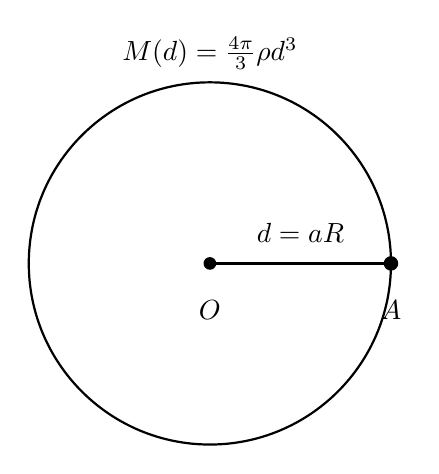
\begin{tikzpicture}[scale=1.15]
\draw[thick] (0,0) circle (2);
\fill (0,0) circle (0.07);
\fill (2,0) circle (0.08);
\draw[thick] (0,0) -- (2,0);
\draw (1,0.12) node[above] {\(d=aR\)};
\draw (0,-0.3) node[below] {\(O\)};
\draw (2,-0.3) node[below] {\(A\)};
\draw (0,2.32) node {\(M(d)=\frac{4\pi}{3}\rho d^3\)};
\end{tikzpicture}\caption{Reduktion nach Newton. Für die Beschleunigung der Galaxie \(A\) heben sich die äußeren Schalen auf; die innerhalb des Radius \(d\) eingeschlossene Masse wirkt, als wäre sie im Punkt \(O\) konzentriert.}\label{fig:c01-newton-sphere}\end{figure}

Bei einer kugelsymmetrischen Massenverteilung verschwindet die resultierende Kraft der Materie außerhalb der Kugel durch \(A\). Die Materie im Inneren wirkt, als wäre sie im Zentrum konzentriert. Die eingeschlossene Masse ist
\begin{equation}
M(d)=\frac{4\pi}{3}\rho d^3.
\label{eq:c01-enclosed-mass}
\end{equation}
Das inverse Quadratgesetz von Newton liefert dann die Beschleunigung von \(A\):
\begin{equation}
\ddot d=-\frac{GM(d)}{d^2}.
\end{equation}
Mit Gleichung~\eqref{eq:c01-radial-kinematics} gilt
\begin{align}
\ddot a R
&=-\frac{G}{d^2}\left(\frac{4\pi}{3}\rho d^3\right) \\
&=-\frac{4\pi G}{3}\rho d \\
&=-\frac{4\pi G}{3}\rho aR.
\end{align}
Der mitbewegte Radius kürzt sich heraus, sodass
\begin{equation}
\boxed{\frac{\ddot a}{a}=-\frac{4\pi G}{3}\rho.}
\label{eq:c01-acceleration}
\end{equation}
Diese Kürzung ist der Konsistenztest. Jede mitbewegte Galaxie gehorcht unabhängig von \(R\) derselben Gleichung für denselben Skalenfaktor.

Setzt man Gleichung~\eqref{eq:c01-density-dilution} ein, erhält man eine der beiden äquivalenten Formen
\begin{equation}
\frac{\ddot a}{a}=-\frac{4\pi G\nu}{3a^3},
\qquad
\ddot a=-\frac{4\pi G\nu}{3a^2}.
\label{eq:c01-acceleration-nu}
\end{equation}
Die erste Form zeigt die relative Beschleunigung; die zweite stellt \(\ddot a\) frei. \(a\) auf der linken Seite zu belassen, ist eine Konvention und ändert nicht die Physik.

\begin{classroomqa}
\audiencequestion{Der Ursprung war beliebig, doch in der Rechnung zeigt jede Kraft zu ihm hin. Wie kann eine andere Wahl des Ursprungs dasselbe Universum ergeben?}
\lecturerresponse{Die Gleichung beschreibt die Relativbewegung. Wiederholt man die Rechnung um eine andere Galaxie, erhält man dieselbe Gleichung, weil die Homogenität dafür sorgt, dass die eingeschlossene Masse nur vom physikalischen Radius abhängt. Wechselt man in ein beschleunigtes Bezugssystem, das an einer anderen Galaxie befestigt ist, und behält zugleich die auf den ersten Ursprung bezogenen Kräfte bei, muss auch die entsprechende Trägheitskraft berücksichtigt werden. Die Wahl eines zentralen Ruhesystems erspart lediglich diese zusätzliche Buchführung. Das invariante Ergebnis ist Gleichung~\eqref{eq:c01-acceleration}, kein ausgezeichnetes Zentrum. \lecturetimestamp{00:43:56--00:46:58}}
\end{classroomqa}

\begin{classroomqa}
\audiencequestion{Gälte das Ergebnis weiterhin, wenn die mitbewegte Massendichte \(\nu\) von Ort zu Ort variierte?}
\lecturerresponse{Nicht in dieser Form mit einer einzigen Funktion. Die einfache Kürzung setzt voraus, dass \(M\propto d^3\) überall dieselbe Proportionalität hat. Wenn \(\nu\) auf der Mittelungsskala merklich variierte, wären in verschiedenen Bereichen unterschiedliche lokale Dynamiken erforderlich, und ein einziger homogener Skalenfaktor könnte sie nicht mehr beschreiben. Die Homogenität leistet hier wesentliche Arbeit. \lecturetimestamp{00:47:05--00:47:51}}
\end{classroomqa}

\begin{classroomqa}
\audiencequestion{Warum schreiben wir \(\ddot a/a\), statt den Faktor \(a\) auf die rechte Seite zu verschieben?}
\lecturerresponse{Beide Formen sind korrekt. In der Kosmologie schreibt man konventionell die relative Beschleunigung \(\ddot a/a\), teilweise weil sie sich direkt mit der relativen Expansionsrate \(H=\dot a/a\) vergleichen lässt. Multipliziert man beide Seiten mit \(a\), erhält man dieselbe Differentialgleichung. \lecturetimestamp{00:50:36--00:51:29}}
\end{classroomqa}

Gleichung~\eqref{eq:c01-acceleration} schließt ein statisches homogenes Newtonsches Universum aus, das mit gewöhnlicher Materie gefüllt ist. Für einen statischen Skalenfaktor müsste \(\ddot a=0\) gelten, während eine positive Dichte eine negative rechte Seite ergibt. Daraus folgt \emph{nicht}, ob das Universum expandiert oder kontrahiert. Es folgt lediglich das Vorzeichen der Beschleunigung.

\section{Negative Beschleunigung bedeutet nicht Kontraktion}

Die Unterscheidung zwischen Geschwindigkeit und Beschleunigung ist elementar, aber entscheidend. Ein Ferrari, der auf der Autobahn vorwärtsfährt, kann eine positive Geschwindigkeit haben und zugleich mit negativer Beschleunigung bremsen. Ebenso kann für ein Universum gelten:
\begin{equation}
\dot a>0,
\qquad
\ddot a<0:
\end{equation}
Es expandiert, doch die Expansion verlangsamt sich.

Um zu entscheiden, ob sich die Bewegung schließlich umkehrt, vergleichen wir das kosmologische Problem mit einem Testteilchen, das sich radial im Gravitationsfeld der Erde bewegt. Sei \(x\) jetzt der physikalische Abstand des Teilchens von einer zentralen Masse \(M\); dieser ist nicht mit der vorherigen mitbewegten Koordinate verwandt. Newtons Gleichung lautet
\begin{equation}
\ddot x=-\frac{GM}{x^2}.
\label{eq:c01-particle-force}
\end{equation}
Die Beschleunigung zeigt stets nach innen. Ein nach außen geworfenes Teilchen kann sich trotzdem lange oder sogar für immer weiter nach außen bewegen. Ein Teilchen, das sich bereits nach innen bewegt, nimmt eine zunehmend negative Geschwindigkeit an. Das Kraftgesetz allein entscheidet nicht, welche Bewegung eintritt; darüber entscheiden die Anfangsbedingungen.

\begin{classroomqa}
\audiencequestion{Bedeutet \(\ddot a<0\), dass das Universum kontrahiert?}
\lecturerresponse{Nein. Kontraktion bedeutet \(\dot a<0\). Ein negatives \(\ddot a\) bedeutet lediglich, dass \(\dot a\) mit der Zeit abnimmt. Beginnt \(\dot a\) mit positivem Wert, bremst die Gravitation die Expansion; ob es null erreicht, hängt von der anfänglichen Expansionsgeschwindigkeit ab – genau wie das Schicksal eines nach außen fliegenden Projektils davon abhängt, ob seine Geschwindigkeit unter- oder oberhalb der Fluchtgeschwindigkeit liegt. \lecturetimestamp{00:51:30--00:56:18}}
\end{classroomqa}

\begin{figure}[ht]\centering
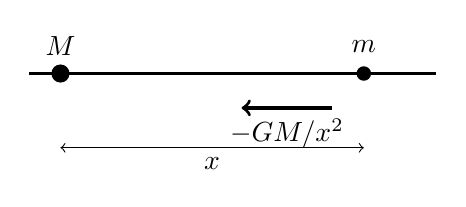
\begin{tikzpicture}[scale=1.15]
\fill (0,0) circle (0.1);
\draw (0,0.3) node {\(M\)};
\draw[thick] (-0.35,0) -- (4.15,0);
\fill (3.35,0) circle (0.08);
\draw (3.35,0.3) node {\(m\)};
\draw[->,very thick] (3.0,-0.38) -- (2.0,-0.38)
  node[midway,below] {\(-GM/x^2\)};
\draw[<->] (0,-0.82) -- (3.35,-0.82)
  node[midway,below] {\(x\)};
\end{tikzpicture}\caption{Das radiale Einteilchenproblem, mit dem sich das Vorzeichen der Beschleunigung von Bewegungsrichtung und weiterem Verlauf trennen ließ.}\label{fig:c01-particle-sketch}\end{figure}

Die Energie macht die Alternativen deutlich. Die erhaltene mechanische Energie lautet
\begin{equation}
E=\frac12 m\dot x^{\,2}-\frac{GMm}{x}.
\label{eq:c01-particle-energy}
\end{equation}
Die potenzielle Energie ist proportional zu \(1/x\), nicht zu \(1/x^2\); die Ableitung von \(-GMm/x\) ergibt die Kraft mit dem inversen Quadratgesetz.

\begin{figure}[ht]\centering
\includegraphics[width=0.82\textwidth]{lecture_01_figure_02.png}\caption{Die Tafel zu Beginn der Energiebetrachtung: eine bewegte Testmasse und ihr kinetischer Term, kurz bevor die gravitative potenzielle Energie wieder hinzugenommen wird.}\lectureframe{00:58:57}\end{figure}

Ist \(E<0\), kann ein nach außen bewegtes Teilchen die Unendlichkeit nicht erreichen, wo seine potenzielle Energie gegen null geht und seine kinetische Energie nichtnegativ ist. Es muss bei endlichem \(x\) anhalten und zurückkehren. Ist \(E>0\), kann es nicht anhalten: An einem Umkehrpunkt wäre die kinetische Energie null und die verbleibende potenzielle Energie negativ, was der Erhaltung einer positiven \(E\) widerspräche. Die Grenze ist
\begin{equation}
E=0,
\end{equation}
und definiert die Fluchtgeschwindigkeit:
\begin{equation}
\frac12 m v_{\rm esc}^2-\frac{GMm}{x}=0,
\qquad
\boxed{v_{\rm esc}^2=\frac{2GM}{x}.}
\label{eq:c01-escape-velocity}
\end{equation}

\begin{figure}[ht]\centering
\includegraphics[width=0.88\textwidth]{lecture_01_figure_03.png}\caption{Die Nullenergiegrenze nimmt an der Tafel Gestalt an. Links sind die früheren kosmologischen Beschleunigungsgleichungen eingerahmt, während rechts das radiale Fluchtproblem entwickelt wird.}\lectureframe{01:01:37}\end{figure}

Genau bei Fluchtgeschwindigkeit wird das Teilchen unbegrenzt langsamer. Seine Geschwindigkeit geht erst für \(x\to\infty\) gegen null; einen Umkehrpunkt bei endlichem Abstand erreicht es nie. Dieser Grenzfall wird das einfachste kosmologische Modell liefern.

\section{Die kosmologische Energiegleichung}

Kehren wir zu einer Galaxie mit festem mitbewegtem Radius \(R\) zurück. Nach dem Schalentheorem ist ihre Radialbewegung identisch mit der eines Teilchens, das sich außerhalb einer Punktmasse bewegt, deren Masse der innerhalb ihrer mitbewegten Kugel eingeschlossenen Masse entspricht.

\begin{figure}[ht]\centering
\includegraphics[width=0.82\textwidth]{lecture_01_figure_04.png}\caption{Die Skizze zur inversen Quadratkraftrichtung und zur radialen Teilchenbewegung, mit der das Energieargument für ein einzelnes Teilchen auf die Kosmologie übertragen wird.}\lectureframe{01:04:14}\end{figure}

Die eingeschlossene Masse nimmt nicht zu, wenn sich die physikalische Kugel ausdehnt. Die Kugel bewegt sich mit, sodass sie stets dieselben Galaxien enthält:
\begin{align}
M
&=\frac{4\pi}{3}\rho(aR)^3 \\
&=\frac{4\pi}{3}\frac{\nu}{a^3}a^3R^3 \\
&=\frac{4\pi}{3}\nu R^3.
\label{eq:c01-fixed-enclosed-mass}
\end{align}
Der erste Ausdruck scheint nur so lange zeitabhängig, bis die Dichteverdünnung berücksichtigt wird. Die Faktoren \(a^3\) kürzen sich heraus.

\begin{classroomqa}
\audiencequestion{Schließt die Kugel mehr Masse ein, wenn sie sich ausdehnt?}
\lecturerresponse{Nein. Ihr physikalischer Radius wächst, aber ihre mitbewegte Grenze bewegt sich mit den Galaxien. Im idealen homogenen Strömungsbild durchquert keine Materie diese Grenze, und Gleichung~\eqref{eq:c01-fixed-enclosed-mass} zeigt die Kürzung ausdrücklich. \lecturetimestamp{01:04:37--01:05:20}}
\end{classroomqa}

Die physikalische Geschwindigkeit der Galaxie ist \(\dot d=\dot a R\), und ihr Abstand vom gewählten Ursprung ist \(d=aR\). Ihre erhaltene Newtonsche Energie lautet daher
\begin{equation}
\boxed{
E=\frac12 m\dot a^{\,2}R^2-\frac{GMm}{aR}.
}
\label{eq:c01-cosmological-energy}
\end{equation}

\begin{figure}[ht]\centering
\includegraphics[width=0.82\textwidth]{lecture_01_figure_05.png}\caption{Die kosmologischen kinetischen und potenziellen Terme an der Tafel. Der vollständige Nenner \(aR\) in Gleichung~\eqref{eq:c01-cosmological-energy} folgt aus dem physikalischen Radius und der zugehörigen Herleitung.}\lectureframe{01:06:12}\end{figure}

Die drei Fälle für die Teilchenenergie entsprechen drei kosmologischen Fällen:
\begin{description}[style=nextline]
\item[\(E<0\):] Die anfängliche Expansion liegt unter der Fluchtgeschwindigkeit; \(a(t)\) erreicht ein Maximum und das Universum kollabiert wieder.
\item[\(E=0\):] Das Universum ist genau kritisch; die Expansion verlangsamt sich für immer und nähert sich der Geschwindigkeit null nur asymptotisch.
\item[\(E>0\):] Die anfängliche Expansion liegt über der Fluchtgeschwindigkeit; im Newtonschen Modell expandiert das Universum für immer und die Rezessionsgeschwindigkeit nähert sich asymptotisch einem von null verschiedenen Wert.
\end{description}

Wir beginnen mit dem Grenzfall \(E=0\). Setzen wir Gleichung~\eqref{eq:c01-cosmological-energy} gleich null, kürzen \(m\) heraus und dividieren durch \(a^2R^2/2\), so erhalten wir
\begin{align}
\frac12\dot a^{\,2}R^2&=\frac{GM}{aR}, \\
\left(\frac{\dot a}{a}\right)^2&=\frac{2GM}{a^3R^3}.
\label{eq:c01-energy-intermediate}
\end{align}
Da
\begin{equation}
\rho=\frac{M}{(4\pi/3)a^3R^3},
\end{equation}
wird Gleichung~\eqref{eq:c01-energy-intermediate} zu
\begin{equation}
\boxed{
H^2=\left(\frac{\dot a}{a}\right)^2=\frac{8\pi G}{3}\rho.
}
\label{eq:c01-first-friedmann}
\end{equation}
Dies ist die erste Friedmann-Gleichung für ein räumlich flaches Universum, das nur Materie und keine kosmologische Konstante enthält; hier wurde sie aus der Newtonschen Energieerhaltung hergeleitet.

\begin{classroomqa}
\classquestion{Was geschieht mit einem Teilchen, das genau mit Fluchtgeschwindigkeit gestartet wird?}
\lecturerresponse{Es wird langsamer, ohne jemals umzukehren. Seine Geschwindigkeit nähert sich erst bei unendlichem Abstand null. Das Universum mit Energie null verhält sich genauso: \(H\) nimmt ab, aber \(\dot a\) bleibt positiv, und es kommt zu keinem Umkehrpunkt nach endlicher Zeit. \lecturetimestamp{01:10:45--01:12:10}}
\end{classroomqa}

Die Faktoren \(4\pi/3\) und \(8\pi G/3\) sind keine willkürliche Dekoration. \(4\pi/3\) ist das Volumen einer Kugel, und der Faktor zwei stammt aus der kinetischen Energie. In der allgemeinen Relativitätstheorie tritt dasselbe \(8\pi G\) in Einsteins Feldgleichung auf, und ihre Zeit-Zeit-Komponente führt zur relativistischen Friedmann-Gleichung. Diese Übereinstimmung ist kein Zufall; die vorliegende Herleitung berücksichtigt jedoch noch keinen Druck, keine räumliche Krümmung als Geometrie und keine kosmologische Konstante.

\section{Die kritische Lösung für ein materiedominiertes Universum}

Verwenden wir das Dichtegesetz \(\rho=\nu/a^3\) in Gleichung~\eqref{eq:c01-first-friedmann}:
\begin{equation}
\left(\frac{\dot a}{a}\right)^2=\frac{8\pi G\nu}{3a^3}.
\label{eq:c01-matter-friedmann}
\end{equation}
Die Konstante \(\nu\) hängt von der willkürlichen Normierung der mitbewegten Koordinaten ab. Um die Zeitabhängigkeit sichtbar zu machen, definieren wir
\begin{equation}
K\equiv\frac{8\pi G\nu}{3}>0.
\end{equation}
Dann gilt
\begin{equation}
\dot a^{\,2}=\frac{K}{a}.
\label{eq:c01-normalized-friedmann}
\end{equation}

\begin{figure}[ht]\centering
\includegraphics[width=0.76\textwidth]{lecture_01_figure_06.png}\caption{Die Friedmann-Skalierung für ein materiedominiertes Universum an der Tafel: zuerst mit ihren Konstanten, dann mit hervorgehobener wesentlicher inverser Potenz des Skalenfaktors.}\lectureframe{01:14:44}\end{figure}

Die rechte Seite von Gleichung~\eqref{eq:c01-normalized-friedmann} ist für jedes endliche positive \(a\) positiv. Für einen Umkehrpunkt müsste \(\dot a=0\) gelten; daher kehrt das kritische Universum seine Bewegung nie um. Seine Expansion wird stetig träger, aber nie so träge, dass sie zum Stillstand kommt.

Lösen wir nun die Gleichung. Man kann die Variablen direkt separieren,
\begin{equation}
a^{1/2}\,da=\sqrt{K}\,dt,
\end{equation}
oder dem Vortrag folgen und ein Potenzgesetz ansetzen,
\begin{equation}
a(t)=Ct^p.
\label{eq:c01-power-trial}
\end{equation}
Dann gilt
\begin{equation}
\frac{\dot a}{a}=\frac{p}{t},
\qquad
\frac{K}{a^3}=\frac{K}{C^3t^{3p}}.
\end{equation}
Einsetzen in Gleichung~\eqref{eq:c01-matter-friedmann} ergibt
\begin{equation}
\frac{p^2}{t^2}=\frac{K}{C^3t^{3p}}.
\end{equation}
Aus dem Vergleich der Potenzen und Koeffizienten folgt
\begin{equation}
3p=2,
\qquad
C^3=\frac{K}{p^2}=\frac{9K}{4}.
\end{equation}
Somit ist
\begin{equation}
\boxed{
a(t)=\left(\frac{3\sqrt K}{2}t\right)^{2/3}\propto t^{2/3}.
}
\label{eq:c01-two-thirds}
\end{equation}
Der additive Zeitursprung wurde so gewählt, dass \(a=0\) bei \(t=0\) gilt. Allgemeiner kann man \(t\) durch \(t-t_0\) ersetzen.

Der Skalenfaktor wächst für immer, während
\begin{equation}
\dot a\propto t^{-1/3}\longrightarrow0,
\qquad
H=\frac{2}{3t}\longrightarrow0.
\label{eq:c01-asymptotic-slope}
\end{equation}
Sein Graph steigt überall an und ist überall nach unten gekrümmt. Er nähert sich keiner horizontalen Geraden, denn \(a(t)\) selbst ist unbeschränkt; seine Steigung geht jedoch gegen null.

\begin{classroomqa}
\audiencequestion{Ergab sich \(t^{2/3}\) nur deshalb, weil dieser spezielle Ansatz zufällig funktionierte? Könnte ein anderer Ansatz eine andere Lösung mit Energie null liefern?}
\lecturerresponse{Der Ansatz identifiziert die Lösung; er liefert nicht bloß eine von mehreren Möglichkeiten. Die Gleichung erster Ordnung für den expandierenden Zweig, \(\dot a=\sqrt{K/a}\), lässt sich bis auf die Normierung und die Wahl des Zeitursprungs eindeutig zu \(a\propto(t-t_0)^{2/3}\) integrieren. Verschiedene Gesamtenergien führen zu verschiedenen Differentialgleichungen und damit zu verschiedenen kosmologischen Entwicklungen. \lecturetimestamp{01:27:07--01:27:43}}
\end{classroomqa}

\begin{classroomqa}
\audiencequestion{Wird die kritische Kurve schließlich horizontal?}
\lecturerresponse{Ihre Steigung geht gegen null: \(\dot a\propto t^{-1/3}\). Dennoch ist sie zu jedem endlichen Zeitpunkt positiv, sodass der Skalenfaktor unbegrenzt weiterwächst. Das Universum nähert sich asymptotisch dem Ruhezustand, ohne ihn zu erreichen. \lecturetimestamp{01:27:48--01:28:57}}
\end{classroomqa}

Dieses einfache Ergebnis ist historisch bemerkenswert. Newton verfügte über die Mechanik und das Schalentheorem, die für diese Herleitung nötig sind, und befasste sich mit Fragen zu einem unendlich ausgedehnten gravitativen Universum; ein expandierendes Modell formulierte er jedoch nicht. In der Diskussion im Hörsaal wurde angedeutet, dass philosophische und theologische Vorstellungen von der kosmischen Geschichte möglicherweise beeinflussten, welche Fragen ihm naheliegend erschienen. Diese historische Vermutung gehört nicht zur Herleitung; der mathematische Punkt ist lediglich, dass die erforderlichen Newtonschen Werkzeuge bereits vorhanden waren.

\begin{classroomqa}
\audiencequestion{Setzt diese Newtonsche Konstruktion ein unendliches Universum voraus?}
\lecturerresponse{Sie setzt einen euklidischen, räumlich flachen Newtonschen Raum voraus. Im üblichen Newtonschen Modell erstreckt sich dieser Raum unbegrenzt, sodass das Modell räumlich unendlich ist, auch wenn sich die Abstände zwischen den mitbewegten Galaxien mit der Zeit ändern. Gekrümmte, endliche räumliche Geometrien gehören zur relativistischen Behandlung. \lecturetimestamp{01:22:12--01:22:55}}
\end{classroomqa}

\section{Jenseits des Nullenergiemodells}

Der Fall mit Energie null ist eine bewusste Vereinfachung, aber nicht das einzige Newtonsche Universum. Behalten wir \(E\neq0\) in Gleichung~\eqref{eq:c01-cosmological-energy} bei, erhalten wir
\begin{equation}
\left(\frac{\dot a}{a}\right)^2
=\frac{8\pi G}{3}\rho+\frac{2E}{mR^2a^2}.
\label{eq:c01-nonzero-energy}
\end{equation}
Homogenität verlangt, dass die Kombination \(2E/(mR^2)\) für jede betrachtete mitbewegte Kugel denselben Wert hat. Bezeichnen wir diesen Wert mit der Konstanten \(C_E\), so gilt
\begin{equation}
H^2=\frac{8\pi G}{3}\rho+\frac{C_E}{a^2}.
\end{equation}
Ein positives \(C_E\) entspricht einer Energie oberhalb der Fluchtenergie; ein negatives \(C_E\) ermöglicht einen Umkehrpunkt. In der relativistischen Notation wird dieser Energieterm im Rahmen der räumlichen Krümmung neu gedeutet – ein Zusammenhang, der der späteren Behandlung vorbehalten bleibt.

Alle drei Materie-allein-Verläufe weisen während der Materiedominanz eine negative Beschleunigung auf:
\begin{equation}
\ddot a=-\frac{4\pi G}{3}\rho a<0.
\end{equation}
Die Kurve für den späteren Kollaps steigt an, erreicht \(\dot a=0\) und fällt dann. Die kritische Kurve \(t^{2/3}\) steigt unbegrenzt weiter, wobei ihre Steigung gegen null geht. Auch die Kurve für positive Energie steigt unbegrenzt weiter und nähert sich einem linearen Wachstum. Eine vorläufige Skizze dieser Fälle an der Tafel wurde während der Vorlesung korrigiert; die gesicherte Schlussfolgerung ist das gemeinsame nach unten gekrümmte Verhalten, nicht jedes Detail der ersten Skizze.

Im beobachteten Universum kommt noch etwas hinzu. Seine frühe, materiedominierte Expansion lässt sich gut durch eine Kurve mit abnehmender Steigung beschreiben, doch zu späteren Zeiten krümmt sich die Kurve nach oben:
\begin{equation}
\ddot a>0.
\end{equation}
Gewöhnliche drucklose Materie kann in Gleichung~\eqref{eq:c01-acceleration} nicht dieses Vorzeichen erzeugen. Dazu ist ein zusätzlicher Term erforderlich. Im einfachsten modernen Modell ist dies eine kosmologische Konstante; allgemeiner spricht man von dunkler Energie. Das vorliegende Kapitel lässt sie bewusst außer Betracht, damit zunächst die Newtonsche Materiedynamik klar verständlich wird.

\begin{classroomqa}
\audiencequestion{Ist das \(8\pi G\) in der Friedmann-Gleichung derselbe Faktor wie in Einsteins Feldgleichung, und haben wir eine kosmologische Konstante berücksichtigt?}
\lecturerresponse{In der allgemeinen Relativitätstheorie tritt dieselbe Gravitationsnormierung auf, und die Zeit-Zeit-Komponente der Feldgleichung ergibt die relativistische Friedmann-Gleichung. Das hier betrachtete Modell enthält keine kosmologische Konstante. Es beschreibt ein materiedominiertes Universum; gerade ein fehlender Term wie der für die kosmologische Konstante kann die Beschleunigung zu späteren Zeiten erklären. \lecturetimestamp{01:30:15--01:31:06}}
\end{classroomqa}

\section{Die mittlere Strömung und lokale Abweichungen}

Die homogene Expansion ist eine Beschreibung auf einer groben Skala. Sie besagt nicht, dass sich jedes Objekt von jedem benachbarten Objekt entfernt. Gravitativ oder anderweitig gebundene Systeme können sich von der Hubble-Strömung entkoppeln. Die Milchstraße und Andromeda nähern sich zum Beispiel einander, statt dem großräumigen Expansionsgesetz zu folgen.

Die Abweichung der Geschwindigkeit einer einzelnen Galaxie von der Hubble-Strömung heißt ihre \emph{Pekuliargeschwindigkeit}. Der Begriff ist fachsprachlich gemeint und kein Werturteil über die Galaxie. Das Hubble-Gesetz ist eine bessere Näherung, wenn man über größere Entfernungen und größere Volumina mittelt. Auf der Skala einer gebundenen Galaxie, eines Galaxienhaufens oder einer lokal überdichten Region können lokale Kräfte gegenüber der Hintergrundexpansion überwiegen.

\begin{classroomqa}
\audiencequestion{Können sich manche Regionen zusammenziehen, obwohl sich das Universum insgesamt ausdehnt?}
\lecturerresponse{Gewiss. Gebundene Systeme und hinreichend dichte Fluktuationen müssen der mittleren Expansion nicht folgen. Das System aus Milchstraße--Andromeda ist ein bekanntes Beispiel. Eine kosmologische Rechnung mittelt über Volumina, die groß genug sind, damit diese Pekuliarbewegungen und lokalen Dichtefluktuationen nicht überwiegen; das Ergebnis \(a(t)\) beschreibt den Hintergrund, nicht jedes Objektpaar. \lecturetimestamp{01:31:00--01:34:13}}
\end{classroomqa}

Die Analogie ist ein gewöhnliches Gas. Wenn man die Luft in einem Raum als gleichförmig bezeichnet, leugnet man damit weder molekulare Fluktuationen noch lokale Dichteunterschiede. Gemeint ist, dass Mittelwerte über hinreichend große Regionen stabil sind. Kosmische Homogenität hat denselben logischen Status, allerdings auf ungleich größeren Skalen. Eine Region, die anfangs etwas dichter als der Durchschnitt ist, kann genügend Eigengravitation aufweisen, um der Expansion zu widerstehen und schließlich zu einer gebundenen Struktur zu kollabieren.

\begin{classroomqa}
\audiencequestion{Kann die Beobachtung entscheiden, ob sich Galaxien durch den Raum bewegen oder ob der expandierende Raum sie auseinanderträgt?}
\lecturerresponse{Nicht, wenn beide Beschreibungen jedem Paar dieselbe Entfernung \(d_{AB}(t)\) zuordnen. In der einen Beschreibung bewegen sich die Galaxien vor einem scheinbar festen Koordinatenhintergrund; in der mitbewegten Beschreibung ruhen die Galaxien, während sich der Skalenfaktor ändert. Beide Beschreibungen sind mathematisch äquivalent. Die allgemeine Relativitätstheorie legt die zweite Ausdrucksweise näher, führt in diesem Vergleich aber keine davon getrennte beobachtbare Größe ein. \lecturetimestamp{01:34:14--01:34:59}}
\end{classroomqa}

\begin{classroomqa}
\audiencequestion{Gibt es neben der Helligkeit von Supernovae vom Typ Ia unabhängige Hinweise auf die kosmische Beschleunigung?}
\lecturerresponse{Ja. Die Schlussfolgerung ergibt sich aus einem Netz von Beobachtungen, insbesondere daraus, wie die Supernova-Messungen und die kosmische Mikrowellenhintergrundstrahlung zusammenpassen. Kein einzelner Messwert trägt die gesamte Schlussfolgerung; entscheidend ist die Übereinstimmung unabhängiger kosmologischer Messungen. \lecturetimestamp{01:35:00--01:35:38}}
\end{classroomqa}

\section{Was gezeigt wurde}

Die Argumentation verlief in einer klaren Reihenfolge:
\begin{enumerate}
\item Großräumige Isotropie legt zusammen mit der Zurückweisung eines ausgezeichneten Zentrums Homogenität nahe.
\item Homogenität ermöglicht ein mitbewegtes Gitter mit einem einzigen Skalenfaktor \(a(t)\).
\item Durch Ableiten des physikalischen Abstands erhält man das Hubble-Gesetz,
  \[
  H=\frac{\dot a}{a},
  \qquad
  v=Hd.
  \]
\item Massenerhaltung in einer mitbewegten Zelle ergibt
  \[
  \rho=\frac{\nu}{a^3}.
  \]
\item Der Kugelschalentheorem von Newton ergibt die Beschleunigungsgleichung
  \[
  \frac{\ddot a}{a}=-\frac{4\pi G}{3}\rho.
  \]
\item Die Energieerhaltung unterscheidet zwischen erneutem Kollaps, kritischer Expansion und ungebundener Expansion.
\item Bei verschwindender Gesamtenergie gilt
  \[
  H^2=\frac{8\pi G}{3}\rho,
  \qquad
  a(t)\propto t^{2/3}.
  \]
\end{enumerate}

Dies ist ein vollständiges Newtonsches Modell eines materiedominierten Universums, aber noch keine vollständige Beschreibung unseres Universums. Es erfasst die Logik der frühen verzögerten Expansion, zeigt, warum ein homogen mit Materie gefülltes Universum nicht statisch bleiben kann, und bestimmt die kritische Expansion an der Grenze zum Entweichen. Energie ungleich null, relativistische räumliche Geometrie, Druck, Strahlung und der für die späte Beschleunigung verantwortliche Term müssen noch hinzukommen.